% a longer version of this was submitted for the ngVLA project as a memo.

%  http://ngvla.nrao.edu/page/memos
%  https://library.nrao.edu/ngvla.shtml

\documentclass[11pt,twoside]{article}
\usepackage{asp2014}
\usepackage{graphicx}
\usepackage{float}
\usepackage{siunitx}


\aspSuppressVolSlug
\resetcounters

\bibliographystyle{asp2014}

\markboth{Teuben}{QAC}

\begin{document}

\title{ngVLA Memo No. 59: \\ QAC: Quick Array Combinations with CASA}
\author{Peter Teuben}
\affil{Astronomy Department, University of Maryland, College Park, MD, USA}

\paperauthor{Teuben~Peter}{teuben@astro.umd.edu}{0000-0003-1774-3436}{Astronomy Department}{University of Maryland}{College Park}{MD}{20742}{USA}

%\aindex{Teuben,~P.~J.}

\begin{abstract}

QAC is a simple python layer in CASA, developed to aid in writing scripts
for array (single dish and interferometric) combinations. Although
initially developed for TP2VIS, running simulations and comparing with
other array combination methods, this package turned out to be useful
for array design studies as well. Both ALMA, ngVLA and CARMA
simulations are already supported, but extending to more generic array
are planned. This memo complements ngVLA memo 54, where
QAC\footnote{this memo describes QAC as of February 2019}
was used for an array design study..


\end{abstract}

%\ooindex{CASA, ascl:1107.013} 

%\ssindex{instruments!interferometer}
%\ssindex{astronomy!radio!single-dish}
%\ssindex{packages!Common Astronomy Software Applications (CASA)}


\section{Introduction}

CASA (\citet{casa1}, \citet{casa2}) 
is a general purpose python interface to radio
astronomy software. It handles interferometric as well as single dish
data, all the way from ingestion, calibration and mapping to
analysis. Most ALMA and VLA data are now routinely processed with CASA
using a custom built pipeline.  CASA Users use object oriented
``tools'', or more classic python functions, called
``tasks'' in CASA. One can write very complex tasks this way, and in fact, the
ALMA/VLA pipeline is an example of such an interface. The QAC
interfaces we discuss in this memo were also designed with a specific
goal of testing the combination of single dish and interferometric data, and
for example are ideal for array design studies.

% The effect of adding short spacings can be dramatic.

% In a previous project, the ADMIT project had a similar challenge, but
% additional more complex boundary conditions.

The development of QAC started in 2017 with the TP2VIS project \citep{tp2vis}, to provide a
more easily programmable interface, orchestrate simulations and provide a
reproducable baseline. It can be obtained from \url{https://github.com/teuben/QAC}.

We first summarize the different methods how CASA can be extended by using your own
custum built python code, then how QAC is installed, and a typical usage. We also give a short
summary of the API, and publish a benchmark in the Appendix. Given that QAC is available
in github, you will likely find updates to QAC (and this memo) in this repository.

\section{Running python code in CASA}

CASA interacts with the user in an interactive python (ipython) session. For most users adding 
C++ code is a complex operation, but installing new python interfaces to ease writing CASA scripts
is usually fairly straightforward, and nowadays most users are familiar with this.
Several methods (and hybrid between these) exist
for CASA:\footnote{some of these methods are expected to become more common in CASA6}


\begin{itemize}

\item[1.] \verb+buildmytasks+

This is the native CASA method. The CASA Cookbook describes a
procedure to install new CASA tasks, but at the same time warns this
method may get deprecated. Nonetheless, this so-called
``buildmytasks'' has been used by other teams, most notably by the Nordic ARC
node\footnote{\url{https://www.oso.nordic-alma.se/software-tools.php}}. This
is typically run once inside the directory where your {\tt foo.py}, {\tt foo.xml},
and other material is present, after which the code, and documentation, gets installed
at the right place inside the CASA tree.

\footnotesize
\begin{verbatim}
    foo(1,'b',[1,2,3])
\end{verbatim}
\normalsize

\item[2.] \verb+import foo+

The traditional way a user includes software to a python based system
would be the python {\tt import} command.
This is fine for stable software, and can be installed with python's
{\tt setuptools} in CASA. In the future CASA6 one should be able to use
virtualenv to test out software like this without the need to write
into CASA's personal space. One can also consider the use of using \verb+$PYTHONPATH+
to point to the directory where {\tt foo.py} is present, but this method can
easily conflict with other installation methods (in fact, is strongly discouraged
in a CASA environment).

%      foo.bar(1,'b',[1,2,3])

\footnotesize
\begin{verbatim}
    foo.bar(1,'b',[1,2,3])
\end{verbatim}
\normalsize



\item[3.] \verb+execfile('foo.py')+

Will execute the code,  after which an API is available  (note this will not work in python3).
This is the method we used in QAC. Notice that no command line parameters can be passed into
the code.

%        foo_bar(1,'b',[1,2,3])

\footnotesize
\begin{verbatim}
    foo_bar(1,'b',[1,2,3])
\end{verbatim}
\normalsize


Incidentally, if these are combined and only one script needs to be executed and then analyzed
outside of CASA, a very efficient way it to use could be to call casa from the command line,
e.g. directly from bash (or via a Makefile):

\footnotesize
\begin{verbatim}
    % casa --nogui -c foo.py a=1 b='"b"' c='[1,2,3]' > foo.log 2&>1
\end{verbatim}
\normalsize

The overhead of setting up CASA before this script really starts work
varies a lot depending on cashing and what's in the casa init files, but can
be anywhere from 5 to 20 seconds. If many of these scripts are to be run, and each
only takes a short time, the overhead is too large, and 





\item[4.]  \verb+run foo.py p1 p2 p3+

Since CASA is essentially an ipython shell, the {\tt run} command can be used to execute
a scripting, including conveniently parsing ``command line arguments''.
This will need a parser for \verb+p1=sys.argv[1]+, \verb+p2=sys.argv[2]+, etc.
note this is an ipython interface, not python, though it's similar to
running in the unix shell \verb+python foo.py p1 p2 p3+, but note this is different
from the CASA method where local python variables can directly be set via the commandline
without the need for a parser.

\footnotesize
\begin{verbatim}
    run foo.py 1  'b'  [1,2,3]
\end{verbatim}
\normalsize

                           
\item[5.]   \verb+%run -m foo+

Runs the foo module (from sys.path). In the current CASA manipulating
{\tt sys.path} is not recommended, the arguments similar to those of not
using \verb+$PYTHONPATH+

\end{itemize}

Miles Lucas made his summer-2019 toolkit Radio Imaging Combination Analysis (RIKA)
available\footnote{\url{https://gitlab.com/mileslucas/RICA}}. He uses the 4th ({\tt run}) method.
In QAC we decided to use the 3rd ({\tt execfile}) method.


\subsection{Installing QAC}

QAC needs CASA to be installed, and the user can opt either to install a version
of CASA from within QAC, or assume a version of CASA that is present on the system, i.e. there
is a existing command called ``casa''. Since CASA startup can be controlled by
\verb+~/.casa/init.py+ we choose this file to {\tt execfile} the correct startup script,
aptly named {\tt casa.init.py} in the QAC distribution:


\begin{verbatim}
    execfile(os.environ['HOME'] + '/.casa/QAC/casa.init.py')
\end{verbatim}

\noindent
There are a few examples of common packages loaded by CASA in {\tt casa.init.py}

\section{Design Issues}

QAC needs to be lightweight, easy to install

\begin{itemize}

\item
  Easy to install, ideally a one liner

\item
  Easy to pass parameters into functions of scripts

\item
  Consistent naming convention of functions and parameters
  
\end{itemize}

\section{Example}

A typical usage would be

\begin{verbatim}
    % casa --nogui -c 
\end{verbatim}


\section{docs}

A typical simulation script might look as follows. Explanations follow later:

\footnotesize
\begin{verbatim}
    qac_ptr(phasecenter,"test123.ptg")
    qac_vla("test123","skymodel.fits", 4096, 0.01, ptg="test123.ptg",
            phasecenter=phasecenter)
            
    qac_clean1("test123/clean1",phasecenter=phasecenter)
\end{verbatim}
\normalsize

\section{Timing and Regression}

Because QAC deal almost exclusively with image type data, the regression test is invoked automatically
with the statistics report, if a regression string (!) is given, viz.

\footnotesize
\begin{verbatim}
r = "0.0038324084555372423 0.021439742878458009 -0.048513446003198624
     0.41929447650909424 383.60327838373536"
qac_stats(test+'/clean/tpint.image')
qac_stats(test+'/clean/tpint_4.tweak.image', r)
\end{verbatim}
\normalsize

where in the first instance only the statistics are reported, the second instance will also flag any deviations.
The numbers represent the mean, std, min, max and total flux of the image.

\section{Benchmarks}

A better supported show of QAC functionality is currently in the **test/bench.py, bench0.py** and **sky1.py** routines [March 2018]
as those were used in the
[SD2018](\url{https://github.com/teuben/sd2018}) workshop. Please note the software in that repo is not maintained anymore,
and updated versions can be found
within QAC.

\section{API}

Here we list the most important functions available in QAC, and a brief explanation where needed. The full and updated
documentation can be seen online on \url{https://github.com/teuben/QAC/blob/master/docs/qac.md}.

\footnotesize
\begin{verbatim}

## Logging

Standard CASA logging is used, and you can use the python **print** function
in the usual way.  You can use the function

    qac_log(msg)

to space your output with a header type message.

Every qac_ command will tag the output with a timestamp, and optionally measure
virtual and real memory. This is added to the standard python **logging** output.
But you must start and end your code as follows:

    qac_begin("test1-alma")
    qac_version()
    ....
    qac_end()


## Simulation routines

As mentioned before,the project directory is within which all the work
occurs. Some routines will accumulate (e.g. qac_vla()), others will
remove that project directory and rebuild that directory
(e.g. qac_clean1). The user will remember to orchestrate them inside
each where needed, e.g.

    qac_vla("test1", cfg=0, ...
    qac_clean1("test1/clean0", ...
    
    qac_vla("test1", cfg=1, ...
    qac_clean1("test1/clean1", ...

    mslist = glob.glob("test1/*.ms")
    qac_clean1("test1/clean2", mslist, ...)


### qac_vla(project, skymodel, imsize, pixel, phasecenter, freq, cfg, ptg, noise)

This is usually how you start a simulation, from a skymodel you create
 a measurement set reprenting a configuration.  Since the ngVLA can
 have multiple configurations, you would need call this routine
 multiple times, e.g.

    qac_vla("test1", cfg=0, ...)
    qac_vla("test2", cfg=0, ...)

Setting different  weights based on dish sizes will need to be implemented. See also qac_alma(). See also
[**simobserve()**](https://casa.nrao.edu/casadocs/latest/global-task-list/task_simobserve/about)

#### input parameters:
```python
qac_vla(project, skymodel, imsize=512, pixel=0.5, phasecenter=None, cfg=1, ptg=None, times=[0.3333333333333333, 1], fix=0, noise=0)
    """
    project     str         working directory for the simulation
    skymodel    str         input image used as a model of the sky. can be CASA image or FITS file
    imsize      int/float   desired skymodel image size in pixels i.e. 512, 1024, 2048, 4096, etc.
    pixel       int/float   desired skymodel pixel size in arcsecs i.e. 1" per pixel, 0.5" per pixel,   etc.
    phasecenter str         the central direction to place the sky model image, or "" or None to use    whatever is in the image already.
    cfg         int         desired ngVLA configuration:
                                        # ant   cfg_name            extent  comments
                            cfg = 0     19      ngvla-sba-revB      < 60m   6m dishes
                            cfg = 1     94      ngvla-core-revB     < 1km
                            cfg = 2     214     ngvla-plains-revB   < 30km 
                            cfg = 3     225     ngvla-gb-vlba-revB  <       [+ 5 25m VLBI dishes, +5 18m    at GBO]
    ptg         str         filename of the pointing file which can be created by qac_im_ptg
    times       list        observation lengths and integration intervals in a list of length 2. times[ 0] = total observation length in hours, times[1] = interval for each integration in seconds. e.g. 4  hour observation with 1 second integrations: times = [4, 1]
    fix         int         if fix=1, removes pointing table. fix=0 is default
    noise       int/float   desired simplenoise (in Jy) to add to the measurement set. default noise=0,     no noise added
    
    """
```

### qac_alma(project, skymodel, imsize, pixel, phasecenter, freq, cycle, cfg, ptg)

Just for kicks, we have way to create ALMA observations from diffent
 cycle's and cfg's. We automatically add a visweightscale to the
 WEIGHT column to properly account for the dish size if you do a
 combination tclean.

### qac_noise(noise, *args, **kwargs)

In the case where you want to empirically set the noise to a certain
 level, this routine will help you determine the proper scaling factor
 for the sm.setnoise() function in simulation tool. So far this is
 only used in qac_vla()

### qac_clean1(project, ms, imsize, pixel, niter, weighting, startmodel, phasecenter, **line)

This is simply a front end to CASA's **tclean()**. Interesting note is
 that **niter** can be a list here, e.g. niter=[0,1000,2000], thus
 creating a series of dirtymaps, showing the progression of clean.

[**tclean()**](https://casa.nrao.edu/casadocs/latest/global-task-list/task_tclean/about)

#### input parameters:
```python
qac_clean1(project, ms, imsize=512, pixel=0.5, niter=0, weighting='natural', startmodel='', phasecenter='', t=True, **line)
    """
    project     str         new working directly as it will be removed before starting
    ms          str         input measurement set to be cleaned. can be single MS or a list
    imsize      int/float   image size in pixels used in the imaging
    pixel       int/float   pixel size in arcsecs used in the imaging
    niter       int         iterations for cleaning. can be single number or a list. niter = 0, no  cleaning done, outputs dirty image
    weighting   str         options for data weighting: natural, uniform, or robust
    startmodel  str         starting model in Jy/pixel
    phasecenter str         mapping center
    t           bool        True means tclean. False means try and fallback to old clean()
    **line                  user can provide any other (t)clean parameters like restfreq or width here
    
    """
```

### qac_tp_otf(project, skymodel, dish, label, freq, template)

Create the OTF map via a simple smooth.

NOTE: **simobserve** also has an **obsmode=sd** keyword, which creates
 a Measurement Set representing the autocorrelations of a TP (sd)
 map. After this you would need to map this MS into a casa image,
 using the
 [**sdimaging()**](https://casa.nrao.edu/casadocs/latest/global-task-list/task_sdimaging/about)
 task.

See Mangum et al.'s (2007) paper :
 https://www.aanda.org/articles/aa/pdf/2007/41/aa7811-07.pdf

### qac_tp_vis(project, imagename, ptg, pixel, niter, phasecenter, rms, maxuv, nvgrp, fix, deconv, **line)

TP2VIS method. Not covering here yet. Like qac_alma(), you can reset the pixel size here.


### qac_feather(project, highres, lowres, label, niteridx)

Feather two maps that were created from qac_clean1 and qac_tp_otf

### qac_ssc(project, highres, lowres)



### qac_smooth(project, skymodel, label, niteridx)

Smooth a skymodel so it can be compared to a (feathered for now) map.


## Helper routines

### qac_stats

### qac_beam

### qac_tpdish

This will depend on fixing the vpmanager interface to tp2vis, but this
 is where you define a new dish size to override the default ALMA 12m
 model

### qac_phasecenter

### qac_ptg

We should re-import the qac_im_ptg routine from qtp. See below.

### qtp_im_ptg(phasecenter, imsize, pixel, grid, im=[], rect=False, outfile=None)

this should possibly become an qac_im_ptg 

### qac_summary

### qac_math

Just a super simple front-end to immath, so we can wrote code such as

    qac_math(out, in1, '+', in2)

it only allows the four basic operators combining two maps. Partially
 driven because immath does not have the overwrite=True option.

### qac_mom

Compute moments 0,1 (and soon 2) in some standard way, so we can
 compare simulations and skymodels.

[**immoments()**](https://casa.nrao.edu/casadocs/latest/global-task-list/task_immoments)

### qac_plot(image, box, plot)

Create a simple colorimage from a casa imasge. By default it appends "png" to the current name.

### qac_flux(image, box, dv, plot)

Create a plot showing flux as function of channel. Good to compare
 flux comparisons between various simulations and skymodels.

### qac_fidelity(model, image, figure_mode=5, diffim=None, absdiffim=None, fidelityim=None, absmodelim=None, interactive=False)

Calculates the fidelity between a model and observed image.



\end{verbatim}
\normalsize


\section{Future}

CASA is a development project, the next
release will have a major overhaul how python and the C++ libraries
are integrated, and this will likely have some effect how QAC is
installed, although less on its API. 

\acknowledgements Jordan Turner and Sara Negussie have been patient contributers and users.
Part of QAC was developed under the ALMA development study ``TP2VIS''  (PI: Jin Koda) and
the ``ngVLA'' array combination study (ngVLA memo 54).

\bibliography{qac}

\newpage
\section*{Appendix A: Sample Code}


To run a large suite of simulations, it can be very useful to call CASA from the Unix command line,
and loop over many parameters, e.g.

\footnotesize
\begin{verbatim}
  casa --nogui -c vla1.py pixel_m=0.05 niter='[0,5000,15000]' dish=45 pdir='"exp102"' 
\end{verbatim}
\normalsize

As one of the products of the ``tp2vis'' ALMA development study (\citet{tp2vis})
we continued the development of the
Quick Array Combination (QAC) toolkit that simplifies writing some of these complex scripts. It also allow us
to use a different combination
method (feather, tp2vis, ssc etc.) with minimal changes to the simulations scripts.

As an example, consider the {\tt simplenoise} procedure to add a given noise to a simulation.
Here is the example calling {\tt qac\_vla()} twice, in the end generating a Measurement Set with
the correct 1 mJy/beam noise:

\footnotesize
\begin{verbatim}

 rms = 0.002                               #  request 2 mJy/beam RMS noise (NA)
 ms1 = qac_vla(pdir,model, noise=-rms)     #  noise<0 triggers it to compute the rms
 sn0 = qac_noise(noise,pdir+'/noise', ms1) #  get scaling factor from rms in ms1
 ms2 = qac_vla(pdir,model, noise=sn0)      #  MS that with correct "rms" in Jy/beam
\end{verbatim}
\normalsize

In the first Measurement Set a noise level is computed for a fixed 1 Jy noise per visiblity on a
zero model. The noise in the resulting dirty map, computed in {\tt qac\_noise()}, is then the scaling factor ({\tt sn0}
that needs to be applied to get the correct requested noise level in the second Measurement Set.








% figures
\newpage

\begin{figure}
\centering
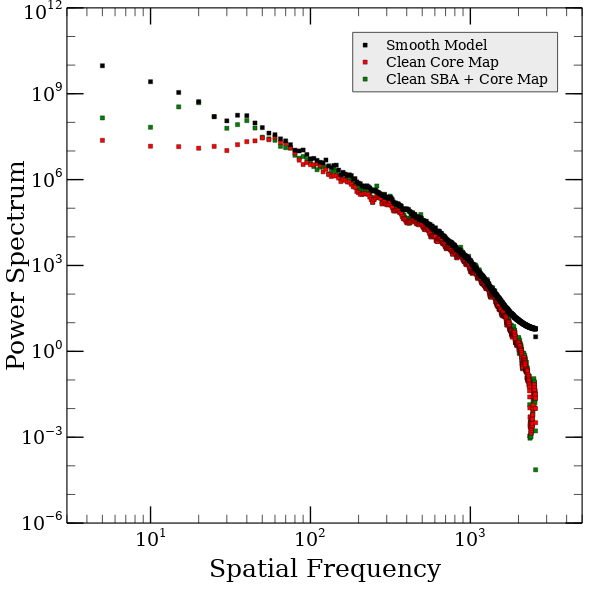
\includegraphics[width=0.49\columnwidth]{figs54/psd1_revised.png}
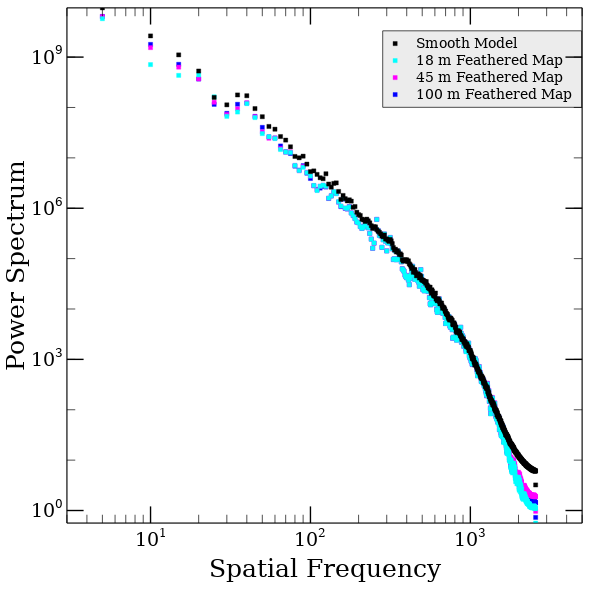
\includegraphics[width=0.49\columnwidth]{figs54/psd2_revised.png}
\caption{Power spectrum density as compared to the smoothed input model (black squares). The left figure shows the power spectrum for the cleaned image with just the ngVLA Core (red) and the cleaned image with both the short baseline array and the core (green). The right figure shows the total power and interferometric feathered images for each single-dish tested: \SI{18}{\meter} dish (cyan), \SI{45}{\meter} dish (magenta), and \SI{100}{\meter} dish (blue).}
\label{fig:psd}
\end{figure}





\end{document}
